%% Using LaTeX-Boilerplate by Adrian-Tudor Panescu %%
%% https://github.com/adrianp/latex-boilerplate %%

\documentclass[12pt,a4paper,twoside]{report}

\def\pdfshellescape{1} % for epstopdf


\usepackage[utf8]{inputenc}
\usepackage[british]{babel}

\usepackage{algorithm}  % in texlive-science
\usepackage{algorithmic}
\usepackage{amsfonts}
\usepackage{amsmath}
\usepackage{amssymb}
\usepackage{appendix}
%\usepackage[T1]{fontenc}
\usepackage{caption}
\usepackage[left=2cm,right=2cm,top=2cm,bottom=2cm]{geometry}
\usepackage{graphicx}
\usepackage{hyperref}
\usepackage{listings}
\usepackage{makeidx}
\usepackage{pdfpages}
\usepackage{placeins}
\usepackage{standalone}
\usepackage{subcaption}

\usepackage{epstopdf}  % load after graphic[s,x]

%% bold float labels
\DeclareCaptionLabelFormat{myformat}{\textbf{#1}~\textbf{#2}}
\captionsetup{labelformat=myformat}

%% detailled margin sizes
%\addtolength{\textwidth}{4cm}
%\addtolength{\oddsidemargin}{-1.5cm}
%\addtolength{\evensidemargin}{-1.5cm}
%\addtolength{\textheight}{4.5cm}
%\addtolength{\topmargin}{-3cm}
%\setlength{\parindent}{0pt}
%\setlength{\parskip}{1ex}

%% Section number format
\renewcommand*\thesection{\arabic{section}}

%% Give numbers to subsubsections and add them to index
\setcounter{secnumdepth}{3}
\setcounter{tocdepth}{3}

%% rename index with care for babel package
\addto\captionsbritish{%
  \renewcommand{\contentsname}%
  {Table of Contents}%
}

%% special table cell that allows line breaks
\newcommand{\specialcell}[2][l]{%
  \begin{tabular}[#1]{@{}c@{}}#2\end{tabular}}

%% do not split long footnotes over multiple pages
\interfootnotelinepenalty=10000

%% uncomment to add a DRAFT watermark on all pages
%!TEX root=../main.tex

\usepackage[printwatermark]{xwatermark}
\usepackage{xcolor}
\usepackage{tikz}

\newsavebox\mybox
\savebox\mybox{\tikz[color=red,opacity=0.1]\node{DRAFT};}
\newwatermark*[
  allpages,
  angle=45,
  scale=10,
  xpos=-20,
  ypos=15
]{\usebox\mybox}


\begin{document}

  \pagenumbering{roman}

  %!TEX root=../main.tex

\maketitle


  % blank pages are inserted for two-side printing
  %!TEX root=../main.tex

\thispagestyle{empty}
%\addtocounter{page}{-1} % do not count this page
\newpage
\mbox{}
\pagebreak


  \begin{abstract}
    %!TEX root=../main.tex

This project aims at enhancing the scientific user community features related
to shared commenting and annotating of scientific literature and data
resources.  The current commenting practices in digital repositories often
cover global, per-document commenting options only. Within the Large Hadron
Collider experiment collaborations at CERN, more targeted needs include
per-section, per-line, or per data item commenting granularity.

In the context of Invenio, a digital library platform originating in the
high-energy physics community, a framework which allows annotating various
types of data resources has been developed. By leveraging it, a general Web
page annotator, and a targeted document commenting system, which allows
referring to specific elements such as pages, sections, figures, or
mathematical equations have been delivered.

State of the art technologies have been employed in order to deliver solutions
which are in line with current Web application practices. The framework
includes an annotation dissemination mechanism, which adheres to standards such
as JSON-LD and REST services, and emerging specifications such as the Open
Annotation RDF data model.

  \end{abstract}

  \cleardoublepage

  \tableofcontents
  \listoffigures
  %\listoftables
  %\lstlistoflistings

  % next page will be odd-numbered (assumes \FloatBarrier)
  \cleardoublepage

  \pagenumbering{arabic}

  \section{Introduction}
    \label{sec:intro}

    \subsection{Invenio Digital Library Platform}
      \label{sec:invenio}
      %!TEX root=../../../main.tex

Invenio \cite{ref:invenio} is a software suite which allows running an online,
large-scale document repository or digital library. Its features cover all
aspects of such repositories, including document ingestion, classification,
ranking, indexing, curation and dissemination \cite{ref:kaplun, ref:glauner};
the architecture of the software is highly modular, each component being in
charge of one the mentioned aspects or other additional features. Currently, it
is being developed by an international developer community and is released as
open source software under the GNU General Public License version two.

Invenio complies with domain-specific standards such as the Open Archives
Initiative (OAI) metadata harvesting protocol. This is a low-barrier mechanism for
repository interoperability, in which HTTP requests can be made to providers in
order to request bibliographic record metadata \cite{ref:oai}.

The software platform is built using the Python programming language and
currently supports the MySQL relational database. Records are represented
internally using a Extensible Markup Language (XML) derivative of the MARC 21
bibliographic format, which is widely used for the representation and exchange
of bibliographic, authority, holdings, classification, and community
information data in machine-readable form \cite{ref:marc}.

The Invenio project originated in the world of high-energy physics, being used
in production by both the CERN Document Server (CDS) and the INSPIRE repository
which is curated by a collaboration of scientist from the Deutsches
Elektronen-Synchrotron, Fermi National Accelerator Laboratory, and SLAC
National Accelerator Laboratory. Nevertheless, the continuous evolution of the
project made it suitable for other use-cases, such as the scientific
information portal of \'{E}cole Polytechnique F\'{e}d\'{e}rale de Lausanne, the
Labordoc document repository of the International Labour Organisation, or the
European Open Access implementations OpenAIRE and ZENODO\footnote{More
information about repositories using Invenio can be found at
\url{http://invenio-software.org/wiki/General/Demo}}.


      \subsubsection{CERN Document Server}
        \label{sec:cds}
        %!TEX root=../../../main.tex


    \subsection{Motivation}
      \label{sec:motiv}
      %!TEX root=../../../main.tex

The initial motivation for this project arose from a use-case originating on
CDS.  Here, the record commenting facilities of Invenio are often used by the
high-energy physics collaborations in order to review new papers in their
pre-publishing stage.  These collaborations use special workflows with multiple
commenting rounds for restricted drafts, necessary for amending potential
issues before making research results public \cite{ref:ludmila}.

In order to reference specific parts of the discussed papers, reviewers often
used a format similar to the following:
  \begin{itemize}
      \item \textit{``P1 - equation system is not presumed''}: a correction
          targeting the first page of the draft.
      \item \textit{``P1/L143 - equation system is not presumed''}: a variation
        of the above which also states the targeted text line.
      \item \textit{``Fig. 2 - equation system is not presumed''}: a comment on
        a figure.
      \item \textit{``P1, E2 - equation system is not presumed''}: a comment on
        Equation 2 on the first page.
  \end{itemize}
This format is also employed when the original paper authors respond to the
corrections, as shown in Fig. \ref{fig:comments}.

\begin{figure}[!ht]
  \centering
  \fbox{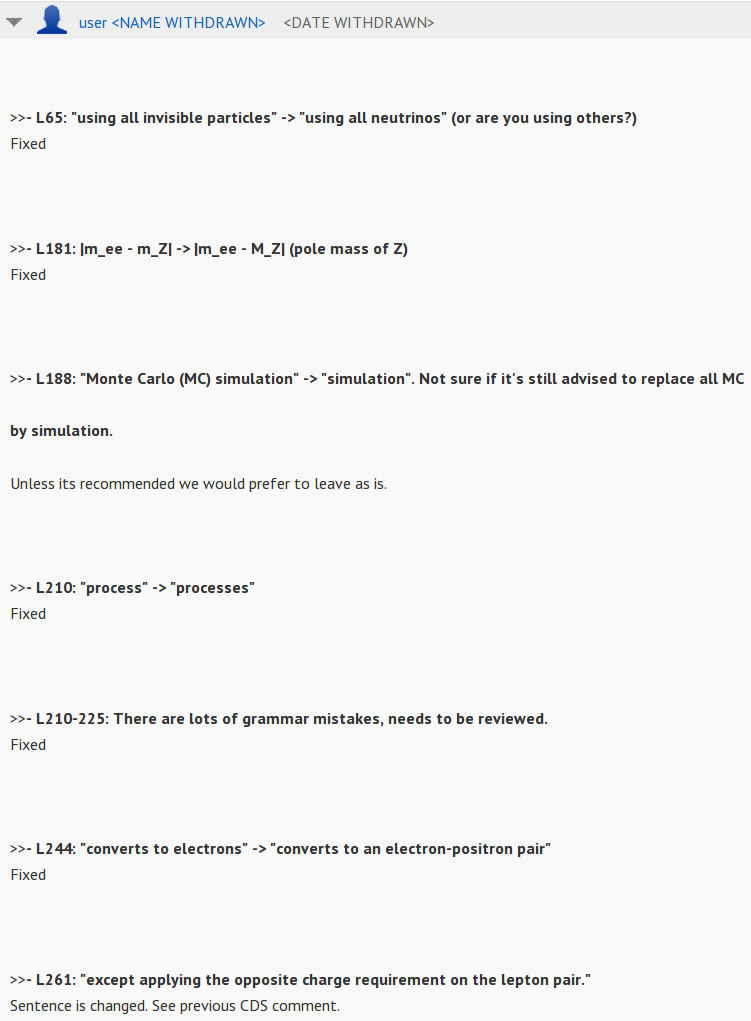
\includegraphics[scale=0.5]{static/img/comments.png}}
  \caption[Example of comments during the paper review phase on CDS]
          {Example of comments during the paper review phase on CDS. The author
           of a paper responds to corrections by referencing text line numbers.}
  \label{fig:comments}
\end{figure}

While being easy to use and clear regarding the corrections, this method also
presents a number of issues:
  \begin{enumerate}
    \item Non-standardised: even within the same commenting round of one draft,
      reviewers used different variations of the markup; for example, to
      reference the first page, both ``P1'' and ``Pag1'' could be used.
    \item Difficult to follow and aggregate: this issue emerged from the
      limitations of Invenio's commenting system which was not purposed for such
      structured input. Namely, both targeted remarks and free textual content
      could be combined in single comments, impeding reviewers from quickly
      identifying the required corrections to be made. Moreover, as commenting
      rounds can consist of hundreds of comments coming from multiple reviewers,
      aggregation is further hindered. For example, in a restricted CDS review
      round, we have identified over one thousand targeted remarks in 180
      comments coming from fifty persons.
  \end{enumerate}
Thus, a solution for solving these issues, while preserving the reviewing
workflow to which the end-users got accustomed to was required.

Aside from pre-publication reviews, such targeted notes could also be seen
useful for annotating resources (textual, multimedia or other formats). While
standard comments are sufficient for discussing general aspects regarding the
content, allowing annotations on various elements such as pages, figures or
paragraphs could prove useful for enriching the content and facilitating its
dissemination. Moreover, while comments often include a social aspect,
annotations could also be used in a private manner, for each user's self study.

Another motivation emerges from the need to consolidate a number of features
present in Invenio and its deployed variants (CDS, INSPIRE) which share a number
of similarities:
\begin{enumerate}
  \item Comments and reviews: allow general remarks on records; reviews include
    a ``\textit{star score}''.
  \item Tags: a new feature to be released in the next major version of Invenio,
    allows users to add brief annotations to records mainly in order to
    organise and categorise them. Can be public, personal to each user, or
    shared between groups.
  \item Baskets: allow users to create collections of records. Similar to tags,
    can be private or shared between users.
\end{enumerate}

Apart from these general Invenio features, certain deployments integrate their
own homologous features. One example is INSPIRE, which implemented a custom
form for allowing users to suggest corrections for the citation list of papers
as the one in Fig. \ref{fig:inspire}. This can be seen as a particular use-case
of the record document review practices previously described, in which only the
reference table is considered.

\begin{figure}[!ht]
  \centering
  \fbox{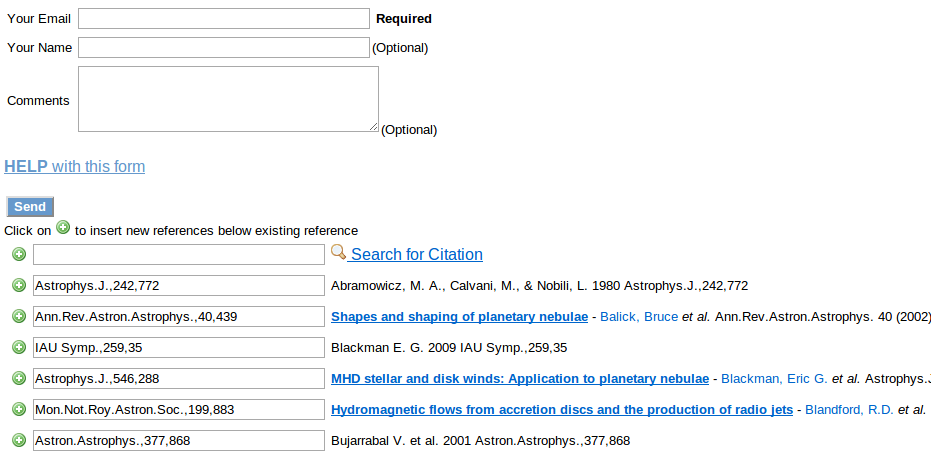
\includegraphics[scale=0.49]{static/img/inspire.png}}
  \caption[Reference correction form as implemented by INSPIRE.]
          {Reference correction form as implemented by INSPIRE. Users are
           invited to suggest amends, a structured form being used for guiding
           data input.}
  \label{fig:inspire}
\end{figure}

A final issue motivating this work is related to the dissemination of metadata.
As mentioned, Invenio already includes features facilitating record harvesting
in compliance with the OAI protocol, but currently does not implement any
specific mechanism for exporting the user-generated metadata.


    %!TEX root=../../main.tex

\paragraph{Thesis Structure} The next section provides an overview on the state
of the art of various commenting and annotating systems, as well as on a number
of technologies for linking data on the Web. Section \ref{sec:design} describes
the conceptual design of the system, and also provides a short account of the
changes scheduled for the next Invenio version, to which this project brought a
number of contributions. Section \ref{sec:impl} details the implementation
aspects and technologies of the annotation solution. The thesis ends with a
number of conclusions and future work possibilities.


  \clearpage

  \section{State of the Art}
    \label{sec:soa}
    %!TEX root=../../main.tex

thepund.it, annotatorjs.org


    \subsection{Commenting and Annotation Systems}
      \label{sec:comments}
      %!TEX root=../../../main.tex

Most Web application nowadays include a social aspect, mostly in the shape of
message forums or commenting capabilities. Apart from platforms fully targeted
at communication among their users, such as message boards, other applications
include facilities that allow commenting the principal features, displayed
content, or simply facilitate user engagement.  Notable examples include most
web blogs, which usually allow comments on posts, YouTube, which encourages
users to discuss videos, or Facebook which augments the social aspect by
embedding comments on all the updates posted by its users.

An emerging trend among web applications is represented by the usage of the
social capabilities of one platform for augmenting another application or
website. For example, Facebook offers the possibility of embedding its widgets,
such that users can comment on external sources using their existing social
network account. A more full-fledged solution in this direction is Disqus
\cite{ref:disqus}, which provides commenting as a service to other
applications, as exemplified in Fig. \ref{fig:disqus}. Such solutions offer
advantages from the points of view of both the application provider and the end
user. The provider saves development time by not having to build a custom
commenting system, while users are given the opportunity to aggregate comments
and annotations generated across applications on various information resources.

\begin{figure}[!ht]
  \centering
  \fbox{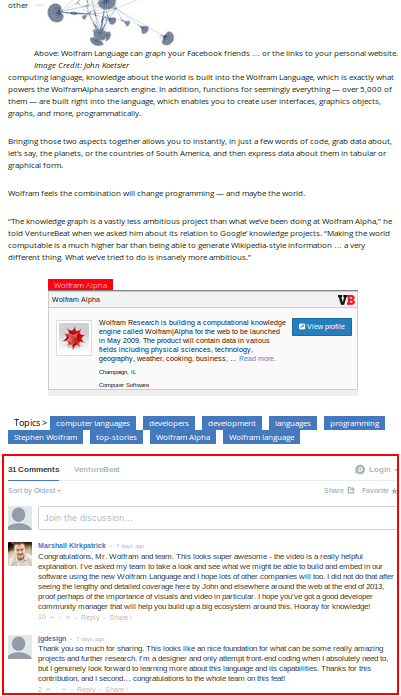
\includegraphics[scale=0.7]{static/img/disqus.png}}
  \caption[Disqus commenting widget embedded on a web blog]
          {Disqus commenting widget (highlighted in red rectangle) embedded on a web blog.}
  \label{fig:disqus}
\end{figure}

Most commenting solutions propose a plain text format for inserting notes, but
alternatives exist. Rich text editors, such as CKEditor \cite{ref:cked} are
often used to allow standard formatting actions (e.g., bold text) on Web forms.
More customisation options can be implemented by using special markup, such as
XML or \LaTeX, which is converted to the target format (e.g., Extensible
HyperText Markup Language (XHTML) for Web applications). Content structure can
be enforced by implementing special forms (see Inspire example in Fig.
\ref{fig:inspire}) or by pre-defining constraints for the users to follow when
inserting plain text (see Section \ref{sec:data} for an example).

While comments satisfy the needs of most applications in terms of social
interaction with and between the end users, they fall short in terms of adding
private notes or enriching existing content by augmenting it with
user-generated material. A trend among the Web community is related to
annotations, which are small pieces of information attached to various
resources, regardless of their type (images, (hyper)text, videos).

Kahan et al. \cite{ref:annotea} proposed the Annotea system, which allows
adding structured notes on Web Documents using the Resource Description
Framework (RDF) format. Annotations are viewed as statements made by the author
about the document. Annotea uses the Amaya \cite{ref:amaya} editor on the
frontend, and a generic RDF database accessible through HTTP server for storage.

The Annotator project \cite{ref:annotator} allows developers to embed a special
widget on their web pages, in order to enable users to annotate any available
textual content, as exemplified in Fig. \ref{fig:annotator}.  It features a
JavaScript front-end, annotations being saved in the JavaScript Object Notation
format in order to be stored on the server side (the reference implementation
features a Python wrapper around Elasticsearch \cite{ref:elasearch}).

\begin{figure}[!ht]
  \centering
  \fbox{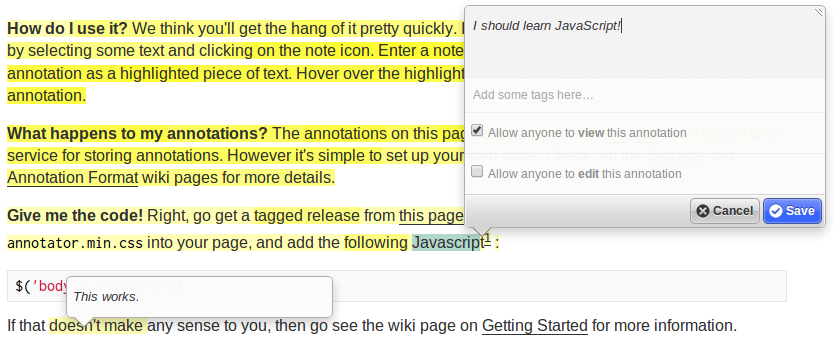
\includegraphics[scale=0.55]{static/img/annotator.png}}
  \caption[Interface of the Annotator project]
          {Interface of the Annotator project. It allows
           adding annotations on any Web page element; in this example, a form
           for annotating a piece of textual information is displayed.}
  \label{fig:annotator}
\end{figure}

While the Annotator project provides a limited number of features, it has an
open plugin interface, which allows third-parties to provide various additions,
such as an image tagging facility, an offline editing mode, or various
visualisation utilities. It is interesting to note that, in contrast to the
commenting solutions discussed previously, this project regards private
annotations as first-class citizens, support for shared content being provided
only by a plugin. While the main purpose of the system is to be deployed over
existing applications, a stand-alone version which allows users to maintain a
collection of annotations over any Web resource is also provided.

A similar project, funded by the European Union's Seventh Framework Programme,
is Pundit \cite{ref:pundit}, which was initially developed in order to enable
humanities researchers to work with manuscripts by leveraging linked data.
Similar to Annotator, it features a JavaScript interface that allows users to
annotate any Web page, but it provides more features in terms of formatting and
structuring the annotations. For example, it allows generating RDF triples, as
exemplified in Fig. \ref{fig:pundit}.

\begin{figure}[!ht]
  \centering
  \fbox{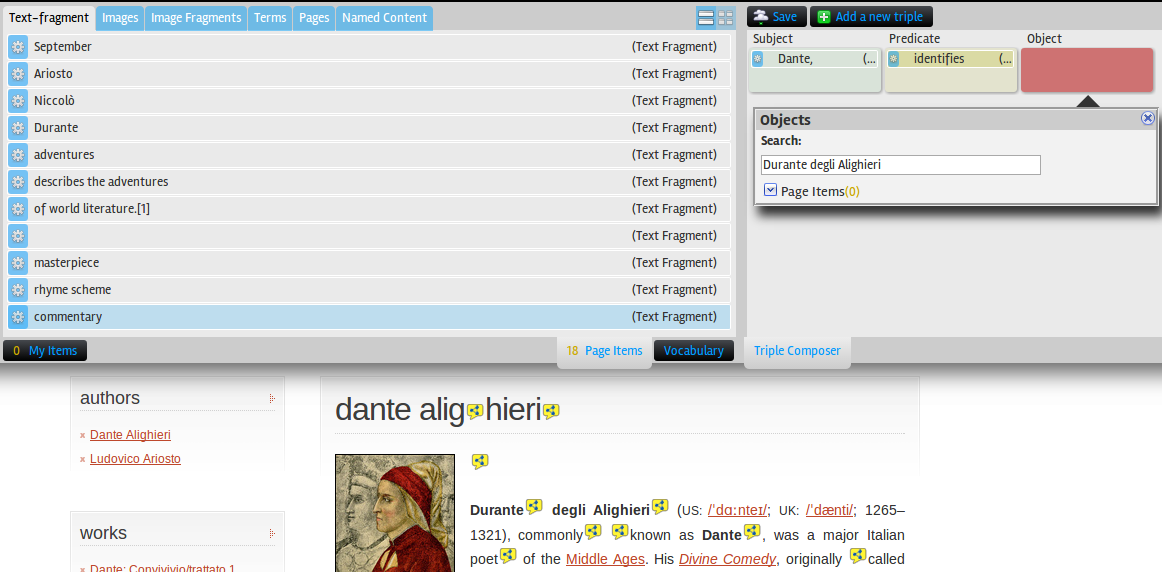
\includegraphics[scale=0.405]{static/img/pundit.png}}
  \caption[Interface of the Pundit project]
          {Interface of the Pundit project. Like Annotator, it allows
           inserting annotations into Web pages, featuring a rich editor
           including RDF triples creation support (right-hand-side), and
           the possibility to link various pieces of information
           (left-hand-side).}
  \label{fig:pundit}
\end{figure}

The main focus of Pundit is allowing users to collaboratively build a knowledge
graph, annotations being targeted not only at augmenting Web pages with
confined information, but also at linking various resources residing on
different domains.

Pundit is designed as a client--server application. The JavaScript client
communicates with the backend through the exposed Representational State
Transfer (REST)\footnote{See Section \ref{sec:pub} for more details regarding
the REST architecture.} interface, which can also be used by third party
plugins.  Annotations are stored in a RDF triple store which exposes a standard
SPARQL \cite{ref:sparql} endpoint. The open nature of the software facilitates
the extension of the platform; for example, video resource tagging was
implemented into Pundit \cite{ref:punditvideo}.

It is important to note that between Annotea and newer projects such as
Annotator and Pundit, the community seemed to move from defining a strict
structure for annotations to a more loose format or to even dropping any
content restrictions. While this might impede the consumption of annotations by
automated systems, it also makes the process more accessible to users allowing
for more metadata to be collected, better reflecting the web resources' meaning
from the users' point of view \cite{ref:wu}.

While the main focus of this project are Web applications, considering the
annotation capabilities of traditional \textit{offline} software is also of
interest. While these applications mostly lack any possibility of linking data
across documents, they also surpass current online applications in terms of
possible methods of highlighting and annotating content. Figure
\ref{fig:xournal} shows a brief usage example of the Xournal open source tool,
which was inspired by Microsoft Windows Journal. Applications such as Adobe
Portable Document Format (PDF) Reader or the Mendeley reference manager provide
similar capabilities, along with the possibility of storing and sharing
annotations online. Moreover, it is worth noting that the interfaces used by
such applications are usually more familiar to users, due to their longer life
span. The resource linking capabilities of online tools along with the
annotation editing capabilities of offline software could prove to be a
powerful combination.

\begin{figure}[!ht]
  \centering
  \fbox{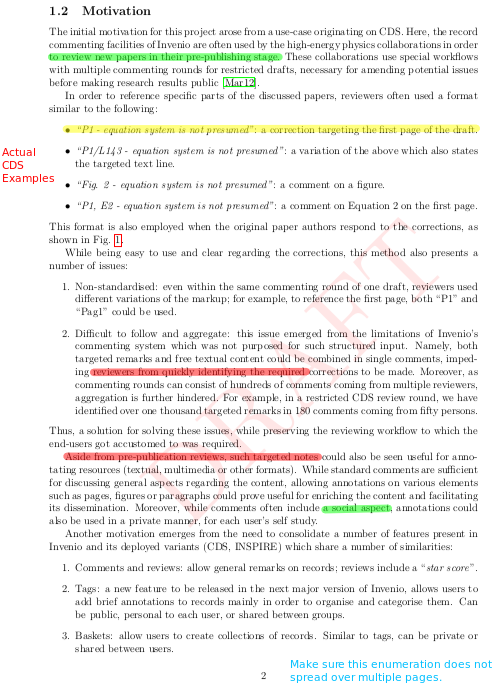
\includegraphics[scale=0.7]{static/img/xournal.png}}
  \caption{Document annotated using Xournal}
  \label{fig:xournal}
\end{figure}


    \subsection{Linked and Structured Data}
      \label{sec:data}
      %!TEX root=../../../main.tex

While annotations facilitate individual note taking for users and improve
engagement inside platforms deploying such mechanisms, it is also desirable
that metadata can be shared across ecosystems in order to allow for new
connections between information resources to be established. Thus, the usage of
standardised annotation dissemination formats is necessary.

The systems presented in the previous section make use of different forms of
RDF structures in order to represent annotations both internally and
externally.  RDF \cite{ref:rdf} is a model defined by the World Wide Web
Consortium (W3C) to be used for online data interchange. The main idea behind
it is related to making statements about resources in the form of
subject--predicate--object expressions, such as:

\begin{verbatim}
  <Dave Beckett> <edits the> <RDF syntax grammar specification>
\end{verbatim}

Due to this structure, these statements are named \textit{triples} in the RDF
terminology.  A collection of RDF statements will constitute a directed
multi-graph, also named the \textit{context} of the concerned triples; contexts
use Internationalised Resource Identifiers (IRI)\footnote{IRI is a
generalisation of Uniform Resource Identifiers (URI), that may contain any
Unicode character; a Uniform Resource Locator (URL) is a type of URI that
identifies a resource through a representation of its primary access
mechanism. Throughout this thesis, only the IRI term will be utilised.} to
link resources. A simple example is shown in Fig. \ref{fig:rdf}

\begin{figure}[p]
  \centering
  \fbox{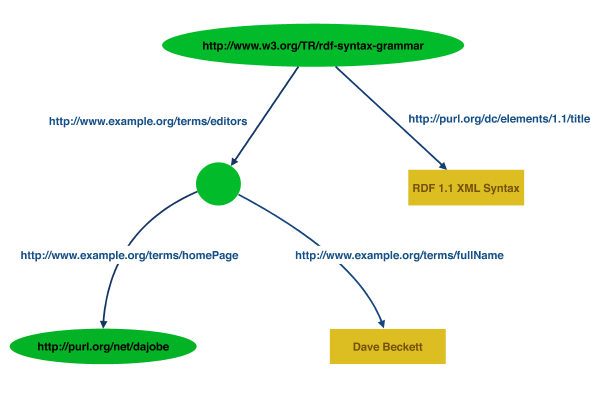
\includegraphics[scale=1]{static/img/rdf.png}}
  \caption[Example RDF graph]
          {Example RDF graph, source \cite{ref:rdfsyntax}. This graph
           can be summarised briefly as: The RDF syntax specification,
           identified by an IRI, has a person characterised by its full name and
           personal Web page as editor.}
  \label{fig:rdf}
\end{figure}

It can be observed that this model is well-suited for the annotations use
case. Metadata can be seen as a statement about a resource in the form (but not
restricted to):

\begin{verbatim}
  <Resource identified by IRI> <has metadata> <annotation body text>
\end{verbatim}

The RDF data model can be serialised in different formats, such as Turtle,
N-Triples, N-Quads (a superset of N-Triples), Notation 3 (N3), RDF/XML or
JSON-LD. Note that the RDF/XML format is commonly referred as simply RDF, due
to its widespread usage, leading to some confusion between the \textit{data
  model} and the \textit{serialisation format}. A typical RDF/XML document will
look as the one in Figure \ref{lst:rdf}, which encodes the graph in Fig.
\ref{fig:rdf}. In order to be encoded in XML, the RDF graph nodes and
predicates need to be represented in the specific structural terms: element
and attribute names, element contents and attribute values. Note that the
example XML uses three collections to define the elements, namely the RDF
standard set, the Dublin Core Metadata Element Set \cite{ref:dc} and a
placeholder set; in real use-cases, each Web application can define its own set
of elements, depending on the specific domain knowledge.

\begin{figure}[p]
  \lstinputlisting[frame=tb,
                   captionpos=b,
                   numbers=none,
                   basicstyle=\ttfamily,
                   showspaces=false,
                   showstringspaces=false,
                   showtabs=false,
                   stepnumber=2,
                   numbersep=4pt]
    {static/lst/rdf.xml}
    \caption[RDF/XML Example]
            {RDF/XML Example, source \cite{ref:rdfsyntax}. Specific XML elements
             are used to encode the RDF context in Fig. \ref{fig:rdf}.}
    \label{lst:rdf}
\end{figure}

Similar to RDF/XML, an augmented version of the JavaScript Object Notation
(JSON) format, JSON-LD, can also be used to serialise the data model; an
in-detail description, in the usage context of the project, is included in
Subsection \ref{sec:json}.

Relational databases, while not suitable for the graph structure of the RDF
model, are commonly used solution for storing such data. If a database stores
only the triples it is called a \textit{triplestore}, and if the context is
also included, a \textit{quad} store is employed. These stores can be queried
using the SPARQL \cite{ref:sparql} language.

\newpage

While RDF provides a standard method for disseminating data, it is mainly
purposed for machine manipulation. Taking the RDF/XML format as an example, it
can be seen that editing such a document by hand is not optimal for end-users.
Nevertheless, capturing input and filling an XML template, while accounting
for invalid data or out-of-scope information, can become expensive in terms of
computing resources.

A simple solution is to deploy standard forms for guiding the users in the data
collection process. The previously discussed Pundit project uses such a visual
form for allowing users to input RDF statements. While this solution is fast to
develop due to the prevalence of the practice in Web applications, it also
lacks in terms of extensibility and scalability; it can be seen that in order
to be able to express complex RDF graphs, a considerable effort must be
invested.

The XTiger \cite{ref:xtiger} XML language allows defining templates, in order
to guide an editing tool for building documents that follow a predefined model.
It does this by pre-defining a set of typed structures and constructors for
these (\textit{components}); for example, a minimal template for inputting
annotations could be defined as in Figure \ref{lst:xtiger}. The XTiger template
can be used to generate documents in target languages, for example XHTML or
RDF/XML.

\begin{figure}[!ht]
  \lstinputlisting[frame=tb,
                   captionpos=b,
                   numbers=none,
                   basicstyle=\ttfamily,
                   showspaces=false,
                   showstringspaces=false,
                   showtabs=false,
                   stepnumber=2,
                   numbersep=4pt]
    {static/lst/xtiger.xml}
  \caption[XTiger template fragment for annotations]
            {XTiger template fragment for annotations. A custom component,
             consisting of two input fields, is defined in the \texttt{xt:head}
             element and used to build the form inside the XHTML body.}
  \label{lst:xtiger}
\end{figure}

\newpage

Special constructs for repeating components across the resulting document can
ease the creation of complex structures. RDF graphs can be constructed by using
the RDF/XML serialisation format as the target for an XTiger template and by
leveraging the special constructs that allow repeating components across the
produced document (e.g., \texttt{xt:repeat}). It is worth noting that XTiger
borrows certain elements from XML Schema, being possible to define the
semantics of XTiger as an extension of XML Document Type Definitions (DTD);
thus the constraints defined by an XTiger template can be expressed in schema
language and an XSLT transformation can be employed to perform the translation
to XML Schema \cite{ref:quint}.

To allow even further flexibility, the Adaptable XML Editing Library (AXEL)
\cite{ref:axel} can be used. This JavaScript library allows users to freely
combine XTiger components, while still producing conforming documents as the
end-result.

Another possibility is to use RDFa \cite{ref:rdfa}, a specification for
attributes to express structured data in any markup language. For example, RDF
attributes can be inserted into the XHTML documents used to present and capture
metadata, facilitating the annotation workflow from both the perspective of the
end-user and the backend system.


      \subsubsection{Open Annotation}
        \label{sec:oa}
        %!TEX root=../../../main.tex

Exporting metadata in a syntactically standard format is a necessary step
towards interoperability between systems collecting user annotations, but not a
sufficient one. The semantics of metadata also need to have an agreed form;
in the context of RDF, applications exporting annotations could also supply an
ontology which describes what the meaning of data is.

The Open Annotation \cite{ref:oa} data model (denoted by \textit{OA} in the
rest of this document) is a specification proposed by W3C that aims at solving
this exact issue. It proposes a general vocabulary of terms that can be used to
describe the most common use-cases of annotations.

The minimal basis of OA is defined as a RDF graph in which annotations have a
target, identified by an Internationalised Resource Identifier (IRI), and a
body; an example graph is included in Figure \ref{fig:oa}. Further restrictions
regarding the types of these elements are not enforced; for example, the target
of an annotation can be another annotation. Nevertheless, it is expected that
the type is specified when serialising the representation, in order to
facilitate third-party consumption.

\begin{figure}[!ht]
  \centering
  \fbox{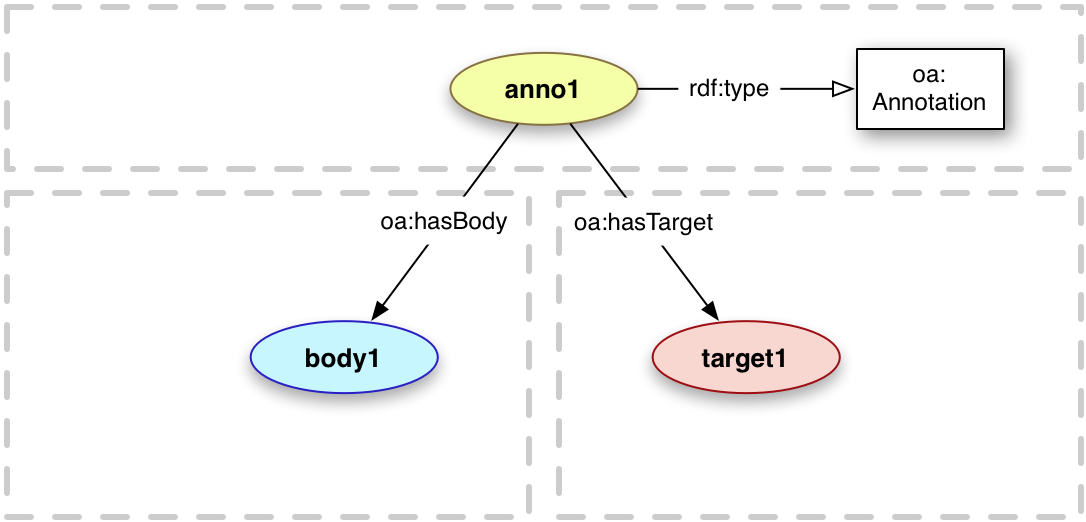
\includegraphics[scale=0.7]{static/img/oa.png}}
  \caption[Basic Open Annotation RDF Graph]
          {Basic Open Annotation RDF Graph, source \cite{ref:oa}. Annotations
           need to specify a body and target identified by an IRI (e.g., a
           Web page).}
  \label{fig:oa}
\end{figure}

\newpage

The body and target attributes can be extended by adding miscellaneous attributes.
For example, Figure \ref{fig:oahubble} presents an annotation where the target
is constrained to a specific region of an image. Similarly, the body can also
be constrained; for instance, it could be specified that only certain pages of
a textbook are describing a target image.

\begin{figure}[!ht]
  \centering
  \fbox{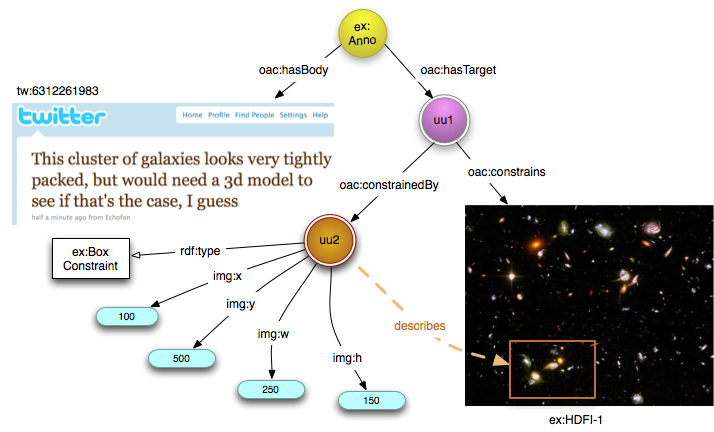
\includegraphics[scale=0.64]{static/img/oahubble.png}}
  \caption[Twitter message used to annotate an image region using Open Annotation.]
          {More complex example usage of Open Annotation, source \cite{ref:oahubble}.
           A Twitter message is used as the body for an annotation targeted at a
           specific region of an image. The \textit{target} attribute points at the whole
           image IRI, but is constrained by rectangle coordinates
           ($x, y, w, h$).}
  \label{fig:oahubble}
\end{figure}

Other elements supported by OA include annotation tagging, versioning the
target or body or constraints on the validity of the annotation (e.g., HTTP
headers than need to be used to retrieve the correct target). Further details
can be found in the specification \cite{ref:oa}.

As Open Annotation model instances are RDF graphs they can be exported in any
of the supported serialisation formats; the guideline is to use JSON-LD
\cite{ref:oa}, the option being further explored by this project, with details
in Section \ref{sec:diss}.


  \clearpage

  \section{System Design}
    \label{sec:design}
    %!TEX root=../../main.tex

Considering the current current features of Invenio and the state of the art, we
have defined the following requirements for adding annotation capabilities to
the platform:
\begin{itemize}
  \item The system should be extensible and allow consolidating the existing
        commenting, reviewing, tagging and grouping of records either by
        superseding the existing feature set or by providing a base framework
        upon which other features can build. Future similar features should be
        considered by means of reducing development time.
  \item The integration of the new system and features should be backward
        compatible and transparent to end-users. Basically, the Invenio
        application should continue to function in the same manner as before
        this project, with identical feature set.
  \item The targeted commenting use-case, presented in Section \ref{sec:motiv}
        should be considered of high-priority, as the described workflow, while
        highly used by the community, is inefficient.
  \item The new system should seamlessly integrate with the access control
        features of Invenio. For example, during the review period, records on
        CDS are restricted to only the participating authors and reviewers.
        Thus, any associated metadata should also obey the access control rules.
  \item Disseminating annotations should be possible in a standardised manner,
        alike the harvesting possibilities employed for records.
\end{itemize}

The first considered option was using one of the systems previously presented,
namely Annotator or Pundit. The first one seems a promising solution, as it
uses a loose data model that can be easily extended to various use cases and
annotation target types. Unfortunately, the software is involved more on the
frontend aspect, with only minimal infrastructure for dissemination and
storage. Also, the project focuses more on annotating fragments of HTML
documents, which does not fit the targeted commenting use case; records in
Invenio provide the full text usually as PDF documents and such, a proper
solution must be implemented in order to allow making references inside them.

The Pundit project is more complete in terms of features, allowing to annotate
various content types out of the box (text, multimedia) and providing a rich
editor which allows embedding RDF graphs and attaching external files. This
option was designed more as a standalone application and not as a lightweight
wrapper like Annotator, providing features such as authentication, or a
complete backend including both storage and dissemination by means of a REST
interface.  This made it unsuitable for a seamless integration with Invenio,
which would have meant stripping any unnecessary components while preserving
the required functionality.

One downside shared by both Annotator and Pundit is related to the targeted
document annotation exemplified in Fig. \ref{fig:comments}. While it is
possible to simulate such a feature in both systems, it is worth noting that
paper reviewers frequently take notes in offline mode (e.g., during commute),
this being one of the reasons behind the employed markup. Using any of the two
systems in offline mode for this purpose is mostly impossible, as they rely on
a rich graphical interface for specifying the exact annotation targets. For
this project's purposes, both an interface and an offline editing mode should
be provided.

The careful evaluation of the existing alternatives lead us to consider
implementing a custom solution which, on one hand, would satisfy all the user
requirements and also allow for a gradual integration in the existing Invenio
framework. Nevertheless, existing components and ideas would be reused and
standard practices would be strictly followed, especially in terms of metadata
dissemination.

The next subsection will give an abstract overview of the proposed system,
while Section \ref{sec:impl} will detail the delivered feature set and
implementation details. Due to the overlap of this project with a major
refactoring of the Invenio project, certain miscellaneous tasks were carried
out in order to provide a working base for the new features; this is briefly
discussed in Subsection \ref{sec:v2}.


    \subsection{Annotation Framework}
      \label{sec:anno}
      %!TEX root=../../../main.tex

For implementing the annotation system, an extensible design was considered, in
which different classes of metadata are constructed using a minimal set of base
elements.  By accounting for the targeted use cases and standard formats, such
as OA, the minimal information set we reckoned necessary for any type of
annotation consists of:
\begin{enumerate}
  \item The target of the annotation (e.g., a document, a Web page, etc.)
  \item The content; we target mostly plain text, with possible markup
        (e.g., \LaTeX), other types, such as multimedia, being possible by
        extending the base models (see below).
  \item The author of the annotation
  \item Time stamp
  \item Permissions of the annotation; arguably, this could also be provided as
        an extension, but as access control is an important aspect of Invenio,
        we considered that all metadata should have restriction rules
        integrated. Public access can also be encoded using this parameter.
\end{enumerate}

Starting from this base, further models can be defined. For example, to allow
attaching external files, only a new field referencing such data needs to be
added. Extensions should also be possible by slightly modifying one of the base
fields; for example, while in the general case the target field is an IRI, for
annotations targeting specific locations in Invenio record documents,
supplementary information (e.g., page number) needs to also be supplied, in the
same manner OA uses constraints. The model is briefly summarised in Fig.
\ref{fig:datamodel}.

\begin{figure}[!ht]
  \centering
  \fbox{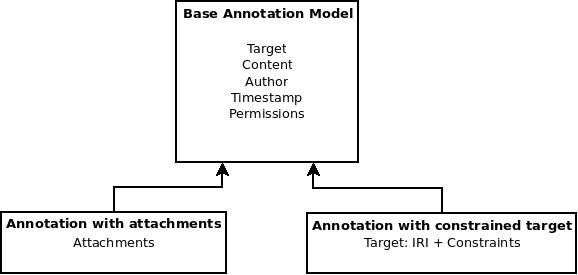
\includegraphics[scale=0.7]{static/dia/datamodel.jpeg}}
  \caption[Basic annotation data model]
          {Basic annotation data model. A series of base fields are defined,
           upon which various annotation types can build more complex
           structures, both by adding new fields or modifying existing ones.}
  \label{fig:datamodel}
\end{figure}

In terms of the system that should provide the annotation facilities, the
following components need to be considered:
\begin{itemize}
  \item Front-end annotation editor; this is presented to end-users,
        who should fill in the target and content fields, the other information
        being assumed. Different annotation models can implement different
        editors, in order to guide users into inputting complete and valid data.
  \item Annotation persistent storage.
  \item Annotation exporter; this should provide access to metadata to third
        parties, in a standardised format and with regard to the access control
        policies.
\end{itemize}
Clearly, seamless communication between these components must be provided,
through an equivalent of the controller in the Model-View-Controller pattern.
Thus, the data flow of the annotation system can be summarised as in Fig.
\ref{fig:dataflow}.

\begin{figure}[!ht]
  \centering
  \fbox{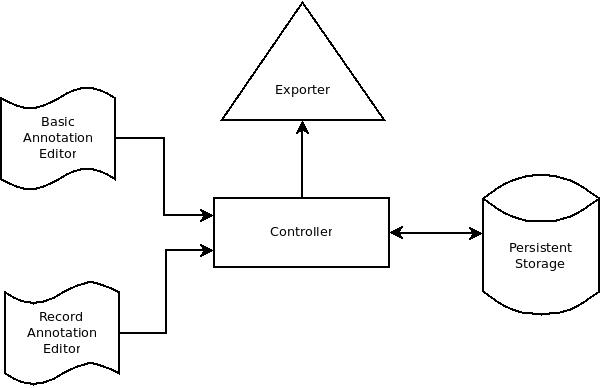
\includegraphics[scale=0.7]{static/dia/dataflow.jpeg}}
  \caption[Annotation system data flow]
          {Annotation system data flow. End-user create new annotations using
           the specialised editors, content being persisted in a database.
           Metadata can be publicised to the interested third parties.}
  \label{fig:dataflow}
\end{figure}

One issue that needs to be considered regarding the extensible annotation model
regards the method used for data persistance. Invenio currently uses a SQL
database, and this model does not fit well the proposed definitions. For
example, if the three models in Fig. \ref{fig:datamodel} are considered, it can
be seen that certain difficulties in expressing them in relational terms will
be encountered. Using separate tables for each model is clearly not optimal in
terms of future scalability, while using one table by, for example, encoding
data in a free text field with a loose syntax, is difficult to maintain,
error-prone, and possibly sub-optimal in terms of system performance.

Fortunately, the new version of Invenio brings support for storing JSON
documents, and the project fully leveraged this possibility, as explained in the
next sections. Apart from solving the issue described above, this method also
facilitates distribution of annotation data to third parties, as JSON is widely
used for these purposes.


    \subsection{Invenio Framework}
      \label{sec:v2}
      %!TEX root=../../../main.tex

As the Invenio software is now being used at large-scale by a considerable
number of organisations across various activity domains, the ability of easily
adapting to various use cases became a stringent requirement. As a result, a
major refactoring of the project, in order to make it more customisable, has
been undertaken. The main focus was on changing the delivery package from a
fairly tightly integrated digital library platform to a coherent collection of
repository components. As this project overlapped with the reorganisation and
contributed a number of required additions and fixes to the main source tree, a
brief description of the process is included in the following.

The first step in rewriting the platform targeted the reorganisation of the
source code. Invenio already featured a modular design \cite{ref:lemeur}, but
further efforts were made to better separate utilities (record commenting, user
messaging etc.) from core bibliographic modules. This also allowed the
identification of components that could be reused outside Invenio, being
general enough for any other Web application. For example, a component offering
support for external user authentication sources is now distributed separately
of core Invenio.

The second important change regards the use of external tools for simplifying
the code base and workflows. A modern framework for building Web applications,
Flask \cite{ref:flask} was employed for replacing the custom Web Server Gateway
Interface (WSGI) components used since Invenio's first iterations. Similarly, a
Structured Query Language (SQL) toolkit and object--relational mapper (ORM),
SQLAlchemy \cite{ref:sqlalchemy}, was employed in order to simplify the code
used for interacting with the database backend and eliminate the need for hand
crafted queries. This is implemented as a thin wrapper around standard Python
classes, that abstracts database operations from developers. An added benefit
of using such a solution is the possibility of switching the database system;
the Invenio collaboration currently explores the move from MySQL to PostgreSQL
for its relational needs.

Other important backend changes involved the data workflow, both inside and
outside Invenio. Support for other formats than MARC was added by a new module,
JSONAlchemy, which is also of interest as it provides abstractions for handling
JSON documents in the same manner SQLAlchemy facilitates the handling of
relational models. Another module that facilitates the creation of REST
interfaces was deployed, a primer usage scenario being an Application
Programmable Interface (API) for document deposition.  Other additions include a
customisable record ingestion workflow engine, developed within the INSPIRE
project, and support for cloud storage by means of a filesystem abstraction
module.

Another targeted aspect relates to the user interface, a modern and
customisable solution being of high interest. Customisability has been achieved
by deploying a templating engine, Jinja version 2, which is already integrated
with the Flask framework, for creating highly modular HTML pages. It features
an extension model in which templates inherit blocks of markup from each other,
similar to object oriented inheritance; thus, if an organisation using Invenio
desires to use its own custom design elements, it just needs to extend or
overload the base templates, modifying only the required parts (e.g., logo or
colour scheme).

Modernisation wise, a series of HTML5 technologies have been employed; the
Bootstrap \cite{ref:bootstrap} frontend framework is being used for defining a
number of interface elements (dialogs, menus, etc.), and updated versions of
various JavaScript libraries for delivering a fluid user experience in line
with modern practices and patterns.

A new deployment process has been developed, replacing the GNU build system
with a Python-specific process for supplying the backend dependencies, and a
specialised workflow for static files, such as JavaScript libraries and style
sheets.

Performance wise improvements were also targeted, indirectly by adopting new
practices while re-witting legacy code, and directly by employing new
technologies such as Redis \cite{ref:redis} for distributed caching, or Celery
\cite{ref:celery} for task scheduling and queuing.

The contributions made by this project to the refactoring are as follows:
\begin{itemize}
  \item Fixed various issues regarding user account handling, such as
        authentication or validation. Also, certain features such as the
        password change facility were ported from the legacy code to the new
        structure.
  \item Contributed with fixes and additions to the developer workflow; for
        example, a brief summary of the steps required for setting up an Invenio
        development environment was compiled and maintained. Certain
        maintenance tasks were also carried out regarding the external
        dependencies used by Invenio, such as version upgrading and source
        discovery and correction.
  \item Improved various user interface aspects, by fixing existing issues,
        further modularising Jinja templates, reorganising source code and
        developing new utilities. For example, a routine for simplifying the
        internationalisation of text strings used inside JavaScript sources
        was developed.
  \item Reorganised the file tree structure for a number of modules, especially
        in regards to better separating JavaScript and Cascading Style Sheets
        (CSS).
  \item Tested the system in order to discover or confirm any issues resulting
        from the code reorganisation, and, where possible, proposed fixes.
\end{itemize}

Apart from these prompt contributions, a number of systematic and more
complex tasks were carried out. As, in the initial phase, the project built
around the commenting facilities already provided by Invenio, this module was
constantly maintained and improved, any general additions being pushed
back to mainline.

\newpage

Other additions have been the result of identifying new requirements while
developing the annotation capabilities, namely:
\begin{enumerate}
  \item Implementing an easy-to-use annotation interface requires displaying a
        preview of the targeted documents, in order to provide the offline
        editor experience described in Section \ref{sec:comments}. While this
        is still an open problem in Invenio, a prototype of such a facility for
        PDF documents has been implemented in the existing previewer module,
        which was also improved to fit the new use-case. A brief research of
        existing solutions was carried out, PDF.js \cite{ref:pdfjs} and Multivio
        \cite{ref:multivio} being considered for future work.
  \item Extending the JSONAlchemy module in order to allow greater
        flexibility in terms of usage scenarios and allow exporting data in
        the JSON-LD RDF serialisation format. This will be discussed further in
        Subsection \ref{sec:diss}.
\end{enumerate}

Finally, in order to provide a demonstrator for the new annotation features, a
special instance of Invenio, Invenio Labs, was deployed at
\url{http://labs.invenio-software.org}. This required maintaining a running
version in an environment close to production ones, while also providing
customisation additions. A significant encountered issue relates to the Python
environment version (2.6) used on CERN servers running the Scientific Linux
operating system. For example, the external library used for generating JSON-LD
documents, PyLD \cite{ref:pyld} was back-ported in order to work properly.

Building this demonstrator was facilitated by the introduction of a new
distinct package, \texttt{invenio-demosite}, which allows developers to quickly
set up a custom Invenio instance. A number of modified HTML templates were
created, a website tutorial feature developed in JavaScript was developed, and
record data along with the necessary deployment routine were put in
place over this standardised customisation package.

The contributions made by this project in terms of source code are
enumerated in Appendix \ref{apx:code}, along with references to the involved
repositories.


  \clearpage

  \section{Implementation}
    \label{sec:impl}
    %!TEX root=../../main.tex

Starting from the requirements and abstract design presented in the previous
section, an implementation of the Invenio annotation facility was proposed,
the next subsections detailing its various aspects.

It is worth noting that due to various constraints, the project started by
implementing the targeted document annotation facility, which built upon the
existing SQL based backend already used for record commenting. The first
iteration was deployed on Invenio Labs, in order to gather information about
possible issues and shortcomings of the design from end-users. Using the
experience gained during this process, the general annotation framework was
developed and the targeted commenting facilities adapting to using it, this
including moving from the SQL backend to a JSON document store based one.

Nonetheless, the description of the developed components will follow the more
logical top--down approach, from the highest level of abstraction to the more
specific use-cases.


    \subsection{General Resource Annotator}
      \label{sec:gra}
      %!TEX root=../../../main.tex

The concrete implementation of the basic annotation model presented in
Subsection \ref{sec:anno} consists of a JSON representation similar to the one
in Fig. \ref{lst:basejson}.

\begin{figure}[!ht]
  \lstinputlisting[frame=tb,
                   captionpos=b,
                   basicstyle=\ttfamily,
                   numbers=none,
                   showspaces=false,
                   showstringspaces=false,
                   showtabs=false,
                   stepnumber=2,
                   numbersep=4pt]
    {static/lst/base.json}
  \caption[Base JSON model for annotations]
          {Base JSON model for annotations; each field is denoted by its name
           and held data type.}
  \label{lst:basejson}
\end{figure}

Each annotation should be distinguished by a Universally Unique Identifier
(UUID) and have its target associated either explicitly or implicitly (through
application specific translations) with an IRI. Other fields include the author
of the annotation (an Invenio user), its textual body, time stamp, and access
restrictions.

This model facilitated the implementation of an annotation system which allows
adding metadata on any Web page of Invenio; users can add such annotations by
using a dialog similar to the one in Fig. \ref{fig:annoform}.

\begin{figure}
  \centering
  \fbox{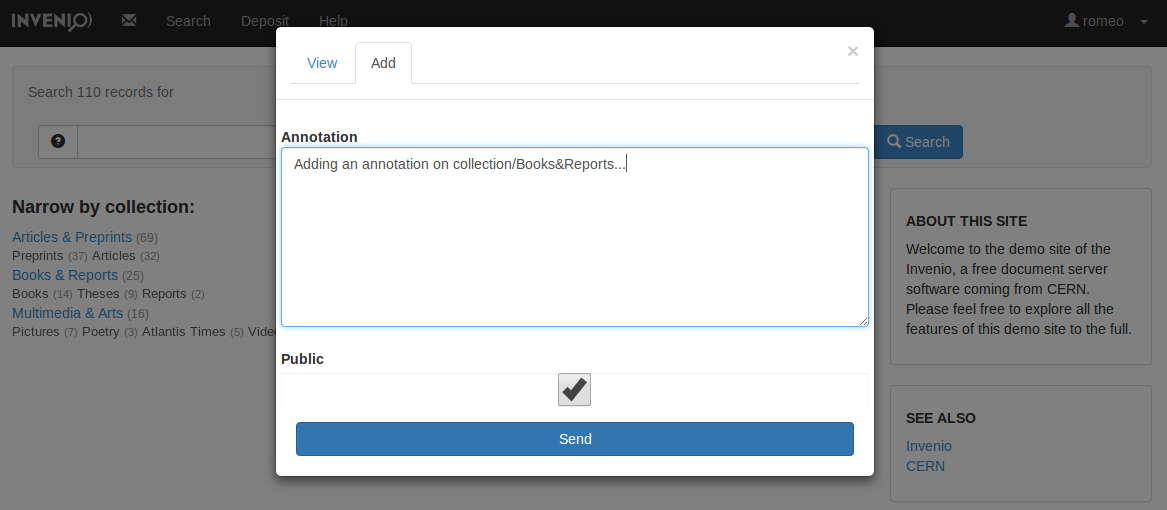
\includegraphics[scale=0.395]{static/img/annoform.png}}
  \caption[Form allowing to add annotations on any Invenio page]
          {Form allowing to add annotations on any Invenio page. Users can add
           add a textual body and specify if the annotation should be public,
           visible to any Web page visitor, or private, visible only to them.}
  \label{fig:annoform}
\end{figure}

The communication between the frontend interface and backend system is mediated
by view functions defined inside a so-called Flask \textit{blueprint}. Apart
from allowing users to input data, displaying annotations is also possible.

Annotations are stored in a MongoDB database \cite{ref:mongo} using the
facilities provided by JSONAlchemy. This module allows defining a schema for
JSON documents, in which the collection of fields and various restrictions on
them can be defined; for example, the UUID is required for all annotations, and
the time stamp should have a standard format. Moreover, JSONAlchemy allows
querying the stored objects (e.g., get all annotations with the target being
the main page of CDS), and modifying them. A thin wrapper for adapting these
operations to the annotation use case is included in an internal API, which can
be used by the Flask blueprint, REST interface (see Subsection \ref{sec:pub}),
or even other Invenio modules to access annotation data. An overview of the
workflow is included in Fig. \ref{fig:baseanno}.

\begin{figure}
  \centering
  \fbox{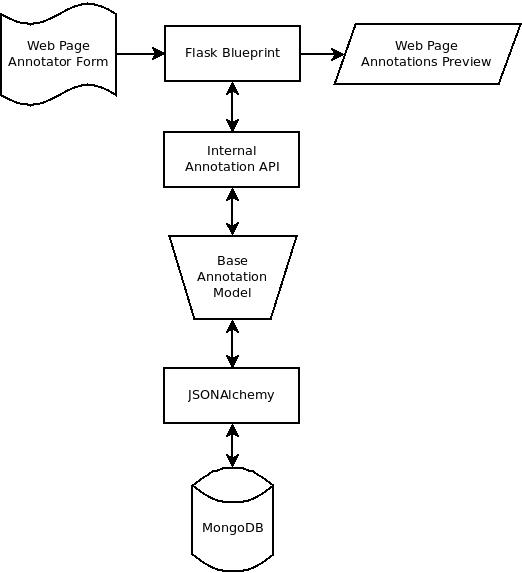
\includegraphics[scale=0.6]{static/dia/base_anno.jpeg}}
  \caption[Web page annotation workflow]
          {Web page annotation workflow; users can add annotations on any
           IRI-identified resource. The specialised API stores data in a
           MongoDB database using the JSONAlchemy model. The Flask blueprint
           provides both annotation creation and display facilities to users
           through its views.}
  \label{fig:baseanno}
\end{figure}


    \subsection{Targeted Document Annotations}
      \label{sec:notes}
      %!TEX root=../../../main.tex

Using the base annotation model as a starting point, the targeted document
commenting feature can be implemented. In this scenario, the \textit{``where''}
field of the base model needs to encode both the document identifier and the
exact target of the annotation (e.g., the second page).

In the current version of Invenio, records can have one or more documents
associated, each of them with multiple versions. For example, during the CDS
paper review rounds, a single record will be used to upload multiple drafts of
the same document. Thus, annotations need to be attached to the correct version
of documents, in order to avoid displaying obsolete information. As the document
storage model is currently changing for the next version of Invenio, we have
chosen to implicitly attach annotations to the latest version of record
documents; nevertheless, this can be changed with minimal effort due to the
customisable nature of the JSON models.

Regarding the document locations to which annotations can refer, after studying
over one thousand comments from CDS review rounds, we have chosen a total of
nine so-called \textit{``markers''} which can identify valid targets:
\begin{enumerate}
  \item Page (P)
  \item Figure (F)
  \item Line (L): this refers to the text line number which is sometimes used
                  in drafts (e.g., \LaTeX\ documents allow this when using the
                  \textit{``draft''} option for the document class). Optionally,
                  this could also be used in other configurations as, for
                  example, specifying a row in a table, or a relative line in a
                  paragraph.
  \item Equation (E)
  \item Table (T)
  \item Section (S): this could also refer to subsections as long as they
                     possess a proper identifier (e.g., Subsection 4.2 can be
                     marked using $S.4: S.2$).
  \item Paragraph (PP): this will likely refer to relative positions, such
                        as \textit{``the third paragraph on the second page''}.
  \item Reference (R): a bibliographic citation, could prove useful in a
                       scenario similar to the INSPIRE reference correction 
                       form presented in Section \ref{sec:motiv}.
  \item General (G): this allows specifying annotations which regard general
                     aspects, such as formatting issues (\textit{``the text is
                     not justified''}), or notes targeting currently nonexistent
                     elements (\textit{``a reference to the 2014 paper needs to
                     be added''}).
\end{enumerate}
The letters between parentheses above denote the special markup that can be
used by users for referring to the various document locations; for example,
\textit{``P.2: F.3a: equation system is not presumed''} is a valid annotation
on subfigure $3a$ on the second page. Markers can be combined to form
hierarchic structures with no depth restrictions; this should facilitate the
specification of precise, unambiguous locations.

This type of annotations can be inserted using the standard Invenio
commenting facilities, in two different manners:

\begin{itemize}
  \item Online, by using the form in Fig. \ref{fig:noteform}, which also
        provides a brief usage tutorial. Moreover, the aggregated view window in
        Fig. \ref{fig:noteview} can be used to point-and-click on the document
        previewer pane to add an annotation on the currently previewed page (the
        input form is pre-filled with the necessary markup).
  \item Offline, by using the described markup to edit the annotations while
        online access to the Invenio instance is not possible. Users can write
        their review, decorate it with the markup and add it later through the
        online form described above in order to be included with the rest of the
        comments. This is the reason for the markup being visible to the users
        and not implicit, directly encoded in the system by means of, for
        example, an interface similar to the one in Fig. \ref{fig:noteview}.
\end{itemize}

\begin{figure}[!h]
  \centering
  \fbox{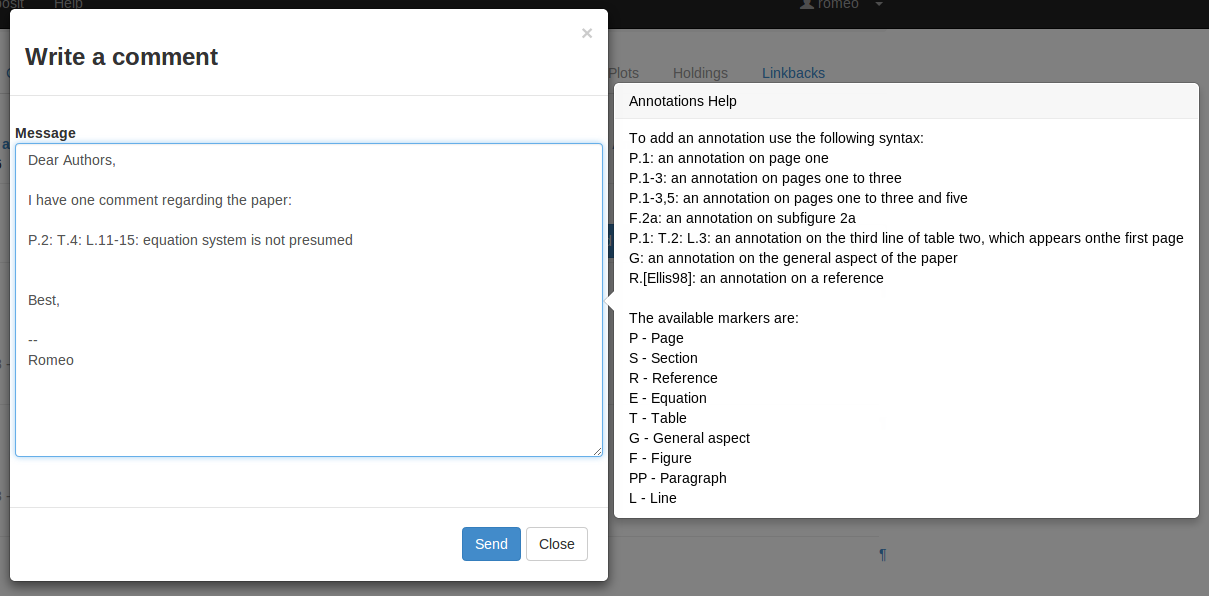
\includegraphics[scale=0.4]{static/img/commentform.png}}
  \caption[Invenio commenting form allowing annotation markup]
          {Invenio commenting form allowing annotation markup. To add remarks
           on any document element users can employ the markup described on the
           right-hand-side.}
  \label{fig:noteform}
\end{figure}

All the added record comments will be scanned and valid annotations will be
extracted by means of a simple regular expression mechanism. From a high level,
annotations are considered valid if complying with the following format:
\begin{verbatim}
  ^<MARKER 1>.<SPECIFIER 1>: [<MARKER 2>.<SPECIFIER 2>: ...
      [<MARKER N>.<SPECIFIER N>:]] <FREE TEXT>$
\end{verbatim}
Square brackets denote optional elements, and the \texttt{\^} and \texttt{\$}
symbols the beginning and end, respectively, of the text line; the line break
is inserted purely for formatting reasons. Specifiers are the actual locations
typed by the markers (e.g., page \textit{one}).

While the final reglar expression used for extracting the annotations is quite
complex, it is composed of simple building blocks. For example, the section
marker is defined in a single line of code, as shown in Fig. \ref{lst:regex}.
Nevertheless, if the regular expression mechanism becomes too complex, or the
user requirements change by including new semantic validation rules (e.g., all
paragraphs need to be specified in relation to a section), the use of a
grammar could be considered.

\begin{figure}[!ht]
  \lstinputlisting[language=Python,
                   frame=tb,
                   captionpos=b,
                   numbers=none,
                   showspaces=false,
                   showstringspaces=false,
                   showtabs=false,
                   stepnumber=2,
                   numbersep=4pt]
    {static/lst/regex.py}
    \caption[Regular expression marker definition for sections]
            {Regular expression marker definition for sections. The regular
             expression is defined as the marker ($S$), followed by a fullstop,
             followed by list of alpa-numeric characters of length equal or
             greater than $1$ (the global definition of $LOCATION$ is currently
             used for almost all markers).}
    \label{lst:regex}
\end{figure}

Extracted annotations will be saved in a JSON document complying with the
JSONAlchemy template, in the MongoDB database. To summarise, the model for
targeted document annotations is similar to the base one presented in Section
\ref{sec:gra}, except for the \textit{``where''} field which is composed of the
record identifier and document marker(s), and a new field containing the
identifier of the comment in which the annotation originated (used for
providing context to end-users). A remark here is that in order to use more
standard IRI locators for the target, as in the base model, a scheme that
allows navigating to a preview of the specified document location could be
used.  For example, \texttt{/record/1/annotations/page1-paragraph2/} could be
employed to open a previewer highlighting the specified text region. This is
currently implemented only for page numbers, due to technical limitations of
the document previewer solution.

For completeness, the workflow of document annotations is included in Fig.
\ref{fig:docanno}.

\begin{figure}[!ht]
  \centering
  \fbox{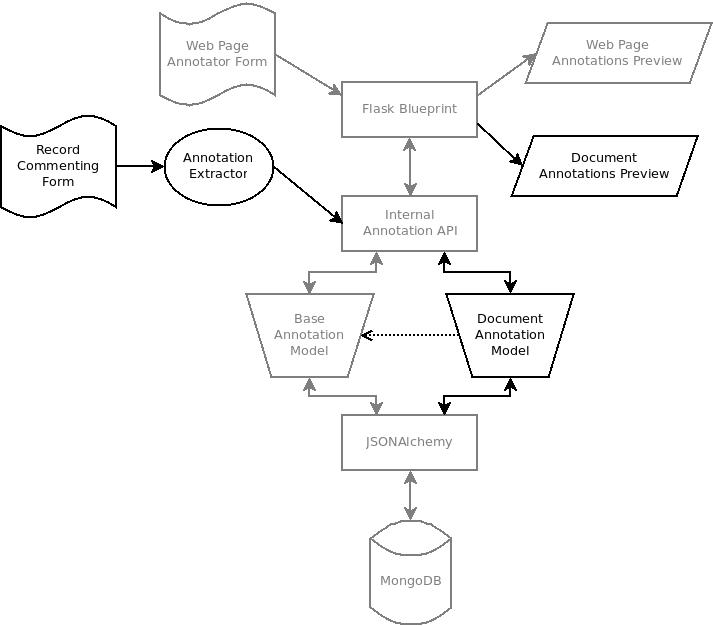
\includegraphics[scale=0.6]{static/dia/doc_anno.jpeg}}
  \caption[Document annotation workflow]
          {Document annotation workflow; the base annotation model is extended
           to allow adding notes on specific document locations (e.g., page,
           figure, equation). Annotations are extracted from basic Invenio
           comments, by identifying the special markup that can be employed by
           users in order to refer to locations.}
  \label{fig:docanno}
\end{figure}

Finally, annotations can be previewed in a manner similar to the one presented
in Fig. \ref{fig:noteview}. The current version proposes a two-column window,
with one column dedicated to previewing the concerned document (currently the
supported format is PDF), and the other to displaying annotations. Coming
back to the CDS review process use-case, the annotation display has been
designed in a manner addressing two issues:
\begin{enumerate}
  \item Separate targeted annotation from free-text comments: even if a comment
        includes both markup decorated and non-structured content, the
        aggregated view will display only the notes targeting a specifying
        aspect. Considering the following comment:
        \begin{verbatim}
          Dear authors,

          This is a very good paper, but I have the following remark:
          P.2: F.3a: equation system is not presumed 

          Regards,
        \end{verbatim}
        only the remark on subfigure $3a$ on the second page will be displayed.
        The complete comments can still be accessed in the standard Invenio
        manner.
  \item Aggregate remarks by location, to allow the authors in charge of
        amending the paper to systematically follow them. As can be observed in
        Fig. \ref{fig:noteview}, annotations are first grouped by page and then
        hierarchically, in a top--down manner, from the most general marker to
        the most particular one.
\end{enumerate}

\begin{figure}[!h]
  \centering
  \fbox{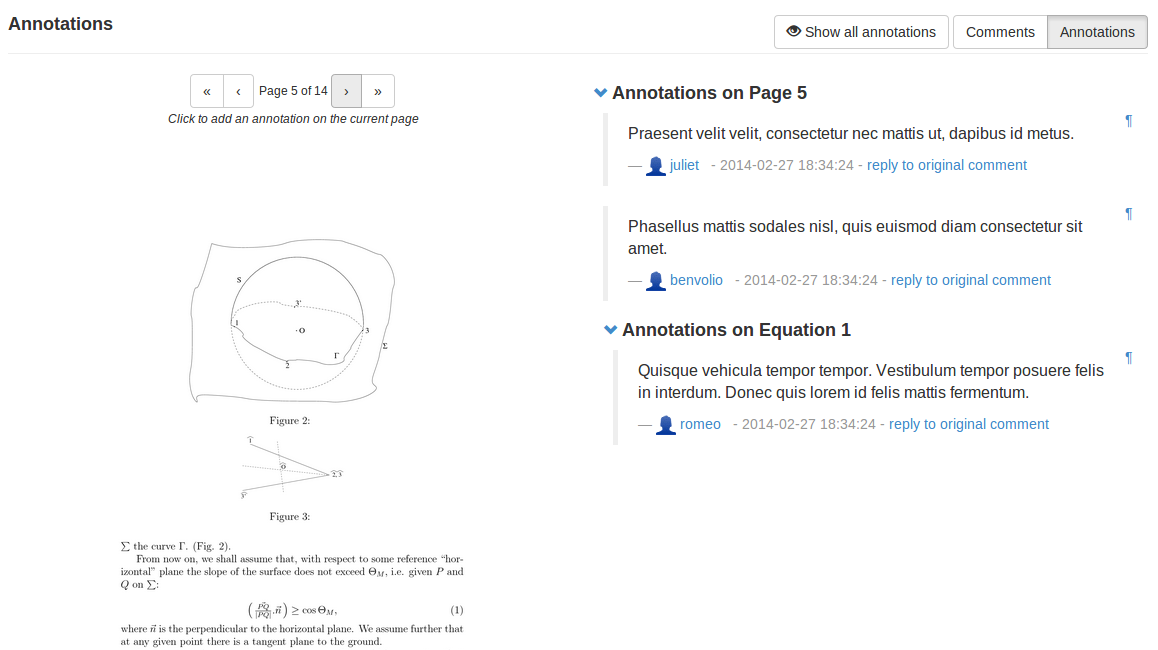
\includegraphics[scale=0.41]{static/img/noteview.png}}
  \caption[Document annotation previewer]
          {Document annotation previewer. A PDF document preview is included on
           the left-hand-side, while the annotations on the currently displayed
           page are presented on the right-hand-side; annotations are
           furthermore aggregated, depending on their sub-markers (e.g.,
           Equation 1). Clicking on the previewer pane allows adding a new
           annotation targeting the displayed page.}
  \label{fig:noteview}
\end{figure}


    \subsection{Dissemination}
      \label{sec:diss}
      %!TEX root=../../../main.tex

As mentioned in Section \ref{sec:oa}, an important capability of most
annotation systems is metadata dissemination. An example use case, related to
the targeted annotation feature, is the routine employed by certain high energy
physics collaborations, which use both CDS and an external wiki application
(TWiki) for their paper review process. Thus, the possibility of transferring
data between applications in a standardised manner could simplify both the
users' workflow and the development process of application providers.

An API that allows exporting annotation data from the Invenio platform has been
implemented and will be described in Subsection \ref{sec:pub}. The system uses
the Open Annotation data model for creating standardised RDF graphs describing
annotations, and exports them using the JSON-LD serialisation format; a brief
description of JSON-LD follows.


      \subsubsection{JavaScript Object Notation for Linked Data}
        \label{sec:json}
        %!TEX root=../../../main.tex

As JSON is a widely used format for transferring Web data, it seems only
natural that a method for specifying linked constructs using it to be proposed.
This is what JSON-LD achieves by allowing to encode RDF graphs in JSON
documents \cite{ref:jsonld}.

For this to be possible, the specification defines a number of keywords, all
preceded by the ``@'' token; the most commonly used ones are:
\begin{itemize}
  \item \texttt{@context}: used to define the keys and possibly values employed
                           inside the JSON document; for example, if JSON
                           is used to describe a person identified by a name,
                           the context could specify that the \textit{``name''}
                           field has the meaning as stipulated in a standard
                           ontology (e.g., Friend of a friend
                           (FOAF) \cite{ref:foaf}). The context is itself a JSON
                           object, where the keys are the various elements used
                           inside the main document and the values are
                           identifiers (e.g., IRI of an ontology).
  \item \texttt{@id}: used to uniquely identify JSON elements, usually by
                      means of an IRI; coming back to the above example, the
                      person could be uniquely identified by a homepage such as
                      \texttt{http://example.com/JohnDoe/}.
  \item \texttt{@type}: used to specify the data type of values (or more
                        generally of RDF nodes); for example, person names have
                        string type.
  \item \texttt{@value}: used to specify the actual data associated with a
                         property in the RDF graph. In the example above, the
                         \textit{``name''} property could have the value
                         \textit{``John Doe''}.
\end{itemize}

\newpage

A JSON-LD document example is included in Fig. \ref{lst:jsonld}. To transform
such a representation to a RDF graph, three simple operations need to be
applied\footnote{The complete algorithm is described formally in the
documentation.}:
\begin{enumerate}
  \item Expansion: this simply removes the context by replacing the keys inside
                   it with the values (usually IRI) across the main object.
  \item Flattening: coverts the JSON object to a list of RDF graph nodes.
                    Basically, it transforms the graph JSON structure into a
                    flat \textit{deterministic} one, in which all properties of
                    a node (identified by \texttt{@id}) are collected in a
                    single JSON object. The resulting graph is represented as
                    a list, the flat structure being easier to parse in an
                    automated manner. Figure \ref{lst:ldflat} provides the
                    flattened version of the document in Fig. \ref{lst:jsonld}.
  \item Conversion: from the flattened form to RDF triples. The result of this
                    final step on the document in Fig. \ref{lst:jsonld} is
                    included in Fig. \ref{lst:nquads}.
\end{enumerate}

\begin{figure}[!ht]
  \lstinputlisting[frame=tb,
                   captionpos=b,
                   numbers=none,
                   basicstyle=\ttfamily,
                   showspaces=false,
                   showstringspaces=false,
                   showtabs=false,
                   stepnumber=2,
                   morekeywords={@context,@id,@type,@value},
                   numbersep=4pt]
    {static/lst/ld.json}
    \caption[JSON-LD document describing a person]
            {JSON-LD document describing a person. The context defines the
             non-keyword elements used within the document, in order to provide
             information to the JSON-LD consumers regarding the semantic
             meaning of data.}
    \label{lst:jsonld}
\end{figure}

\begin{figure}[!ht]
  \lstinputlisting[frame=tb,
                   captionpos=b,
                   numbers=none,
                   basicstyle=\ttfamily,
                   showspaces=false,
                   showstringspaces=false,
                   showtabs=false,
                   stepnumber=2,
                   morekeywords={@context,@id,@type,@value,@graph},
                   numbersep=4pt]
    {static/lst/ldflat.json}
    \caption[Expanded and flattened JSON-LD document]
            {Expanded and subsequently flattened version of the JSON-LD document
             in Fig. \ref{lst:jsonld}. The terms which are not keywords in the
             JSON-LD vocabulary are replaced by their values from the original
             context, and the properties of each RDF graph node are collected in
             a single object. Therefore, the graph (\texttt{@graph}) will
             contain two nodes, one for each person.}
    \label{lst:ldflat}
\end{figure}

\begin{figure}[!ht]
  \lstinputlisting[frame=tb,
                   captionpos=b,
                   basicstyle=\ttfamily,
                   numbers=none,
                   showspaces=false,
                   showstringspaces=false,
                   showtabs=false,
                   stepnumber=2,
                   numbersep=4pt]
    {static/lst/nquads.xml}
    \caption[Information extracted from JSON-LD document in RDF N-Quads format]
            {Information extracted from the JSON-LD document in
             Fig. \ref{lst:jsonld} in RDF N-Quads format. The five statements,
             ended by full stop, specify that the resource identified by the IRI
             \texttt{http://example.com/JohnDoe/} is of type
             \textit{``person''}, with the meaning defined in the FOAF ontology,
             and has the name \textit{``John Doe''}, of type text (string) as
             defined in the Dublin Core Metadata Element Set (see
             \textit{``type''} term in \cite{ref:dc}). Moreover, this person has
             an acquaintance, \textit{``Jane Doe''}, described similarly.}
    \label{lst:nquads}
\end{figure}

Apart from being able to generate RDF graphs, this representation can be used
with another purpose, namely to obtain translated versions of the same data.
Consider a simple example in which a system supplies information about its
users in a format similar to the one in Fig. \ref{lst:jsonld}. Another
application wishes to use this information, but due to its internal workflow,
would need to obtain a JSON document in which the \textit{``name''} property
identifiers are replaced by \textit{``full-name''}.  Clearly, this could be
achieved by retrieving the JSON document from the first system and modifying
the fields, however, JSON-LD API implementations, such as PyLD \cite{ref:pyld},
provide another method, which basically can move the translation step from
consumer- to producer- side.  This method requires supplying another context
when retrieving the expanded (or flattened) JSON document, which specifies the
required translations; coming back to the above example, such a context can be:
\begin{verbatim}
  "@context": {"full-name": "http://xmlns.com/foaf/spec/#term_name"}
\end{verbatim}

Note that in both this context and the original one (Fig. \ref{lst:jsonld}),
the \textit{name} and \textit{full-name} keys, respectively, refer to the same
ontology IRI. Retrieving an expanded JSON-LD through this method, with a
context supplied, is a \textit{compaction} operation; the result will be a new
JSON document, in which the translations specified in the new context will be
applied (\textit{``name''} is replaced by \textit{``full-name''}). If no new
context is supplied, the expanded JSON-LD document is retrieved. This should be
the preferred communication method between applications interchanging JSON-LD
data. It is interesting to note that the specification allows sending an IRI to
a new context through an HTTP Link Header \cite{ref:rfc5988}, thus eliminating
the need for sending large JSON payloads.

While the above examples are trivial, more complex modelling and dissemination
operations can be achieved using JSON-LD. The next subsection gives an overview
on how this technology was employed for publicising annotations.


      \subsubsection{Annotation Publishing}
        \label{sec:pub}
        %!TEX root=../../../main.tex

In order to disseminate annotation data in a standardised manner two issues
need to be considered:
\begin{enumerate}
  \item Format annotations using an established specification.
  \item Provide an easy to use mechanism for data distribution.
\end{enumerate}

Regarding the data format, we have chosen the Open Annotation data model, which
recommends using a JSON-LD RDF serialisation for making annotations public
\cite{ref:oa}. Basically, the specification provides a context, in which the
keys are the various OA model components, and the values IRI to various
ontologies, such as FOAF, Dublin Core Metadata Element Set, RDF, or the specific
OA vocabulary.

This context can be used by applications to convert their own internal
annotation representations to a standard JSON-LD document; if the internal
model is already in JSON form, this can be achieved directly by compaction or
even by modifying the context keys to match to internal ones.

Despite employing a JSON model in our implementation, we have chosen to
programmatically apply the processing steps. Namely, a thin interface over
JSONAlchemy was implemented\footnote{The code for this wrapper is already
included in the source tree of the next Invenio version and will be shipped
separately from the annotation features.}, allowing objects stored in JSON form
to specify their custom translation method. This method uses a default context,
but custom ones can also be supplied, given that the object class has the
required flexibility.

For the annotations, the method will use the OA context and apply a number of
simple conversions. Let us consider the targeted annotations use-case,
described in Section \ref{sec:notes}, for which the conversions are as follows:
\begin{itemize}
  \item The main identifier of the resource is an IRI pointing to an endpoint of
        the Invenio installation which can supply annotations in the internal
        JSON format; this should not be frequently used, but is included for
        completeness. The type of the resource is \texttt{Annotation} in the
        OA vocabulary.
  \item The OA \texttt{annotatedBy} contains information regarding
        the user that created the annotation. Recall that, internally, we store
        only an identifier, which can be used to retrieve all other associated
        information, such as the name or email address. If, instead of applying
        the explicit conversion process, the JSON-LD compaction routine would be
        used, the mentioned information would need to be directly included in
        the annotation JSON model, resulting in duplication of data. Another
        solution would be to provide only minimal information regarding users,
        namely an IRI pointing to a complete profile\footnote{This is currently
        not available in Invenio.}.
  \item For the \texttt{annotatedAt} field, the time stamp is provided as-is. A
        note here is that, as data producers have no knowledge regarding their
        consumers, time zone information, usually as a value denoting the offset
        from the Coordinated Universal Time (UTC), needs to be included.
  \item For the \texttt{hasBody} field, the annotation content is provided, along
        with its format (\texttt{format/plain}) and encoding (Universal
        Transformation Formats--8-bit (UTF-8)).
  \item The \texttt{hasTarget} field is encoded as the IRI to the record of the
        document being annotated, along with a OA \texttt{FragmentSelector}
        data type instance, which specifies to what part of the document the
        annotation refers to (a marker such as \textit{``second paragraph on
        third page''}, encoded in the manner described in
        Section \ref{sec:notes}). Note that if a method of accessing document
        fragments directly through a valid IRI is provided, specifying the
        selector is no longer necessary.
\end{itemize}
For annotations on Invenio Web pages the process is similar, except for the
target field, which can be identified uniquely by an IRI.

The end result of the translation operation is a JSON document which, apart
from the fields described above, also contains the entire context definitions;
this is denoted internally as the \textit{``full''} format. Other formats, such
as the expanded or N-Quads ones, can be obtained by simply calls to the PyLD
library \cite{ref:pyld}. An example of an expanded JSON-LD representation of a
document annotation is included in Fig. \ref{lst:annojson}.

\begin{figure}[!ht]
  \lstinputlisting[frame=tb,
                   captionpos=b,
                   basicstyle=\footnotesize,
                   numbers=none,
                   showspaces=false,
                   showstringspaces=false,
                   showtabs=false,
                   stepnumber=2,
                   morekeywords={@context,@id,@type,@value},
                   numbersep=4pt]
    {static/lst/rest.json}
    \caption[Annotation serialised as an expanded JSON-LD document]
            {Annotation serialised as an expanded JSON-LD document. The internal
             representation is converted to an OA compliant one, using the
             standard vocabulary.}
    \label{lst:annojson}
\end{figure}

Annotation data is served to any interested third-party through a REST Web
interface. At an abstract level, REST is an architectural style in which the
internal system details are ignored, the focus being on the component roles,
the constraints on their interactions, and on the interpretation on significant
data elements.

In terms of Web applications, the REST architecture defines a number of formal
constraints on the client--server communication protocols:
\begin{itemize}
  \item Servers and clients are separated by a uniform interface, each having
        its own distinct set of functions; for example, only servers are
        concerned with data storage, and user interfaces are handled only by
        clients.
  \item Communication is stateless, no client information being stored in the
        server between requests; this requires clients to supply all necessary
        data with each request.
  \item Server responses may be cached and load-balancing may be employed
        without disrupting clients or corrupting data.
\end{itemize}

\FloatBarrier

The uniform server--client interface is the basis of the REST architecture and
can be described in terms of guidelines targeting four aspects:
\begin{enumerate}
  \item Resource distinguishability: resources are uniquely identified (e.g., in
                                     Web applications by IRI) and separated from
                                     their internal structure (e.g., an object
                                     stored in a SQL database will be served to
                                     Web clients in a XML or JSON format).
  \item Resource manipulation: given an object representation, a client holds
                               information to perform any editing or deletion
                               action over the object.
  \item Message description: request responses need to be self-descriptive,
                             specifying the actions clients need to undertake in
                             order to process them. For example, in the case of
                             Web applications, the format of the message (e.g,
                             XML) needs to be included alongside the server
                             response.
  \item Hypermedia as the Engine of Application State (HATEOAS): apart from a
              limited set of simple endpoints, clients do no make any
              assumptions regarding the possible server actions, but only follow
              the hyperlinks provided in request responses. For most Web REST
              interfaces, a brief specification defining the endpoints is
              provided, and clients cannot step outside these boundaries,
              except when receiving explicit instructions from the server.
\end{enumerate}

As previously mentioned, the new version of Invenio provides the basic building
blocks for REST interfaces. Each module that desires to implement such a
facility simply needs to define the endpoints, the methods clients can use to
retrieve data (e.g., \texttt{GET} or \texttt{POST}) and the request template.

For the annotation use-case, one endpoint (\texttt{/api/annotations/export/}),
accepting two request methods (\texttt{GET} and \texttt{POST}) is provided.
Through the \texttt{GET} method clients can get annotation data in a format
similar to the internal one, this being used, for example, to build the IRI
supplied as the main object \texttt{@id} in the JSON-LD representation (see
Fig. \ref{lst:annojson}). The parameters used for this type of request can be
used to perform simple annotation queries; for example, to retrieve all
annotations targeting the first page of any document a request to
\texttt{api/annotations/export/?where.marker=P.1} can be performed.

More complex queries, along with requests to JSON-LD serialisations can be
performed using the \texttt{POST} method. This allows clients to specify the
request parameters in a JSON document in which three parameters are of interest:
\begin{enumerate}
  \item \texttt{query}: used to filter the retrieved annotations; the format is
                        as defined by MongoDB for queries \cite{ref:mongo}.
  \item \texttt{ldexport}: the JSON-LD format to use for serialisation. Can be
                           full, expanded, compacted, flattened, framed (having
                           a custom tree structure, see \cite{ref:jsonldframe}),
                           or normalised (RDF triples).
  \item \texttt{new\_context}: the new context to use for compaction or
                               flattening, the tree structure for framing, or
                               the normalisation options (e.g.,
                               $\{``format'': ``application/nquads''\}$).
\end{enumerate}

To retrieve the document in Fig. \ref{lst:annojson}, the following
query can be used:
\begin{verbatim}
  curl labs.invenio-software.org/api/annotations/export/  \
       -H "Content-Type: application/json"  \
       --data '{"query": {"where.marker": "P.2-PP.3"},  \
                "ldexport": "compacted",  \
                "new_context": {}}'
\end{verbatim}
Recall that JSON-LD expansion and compaction with an empty context are similar
operations.

The proposed mechanism closely follows the REST guidelines: only a minimal set
of simple, unique, endpoints is provided, clients being allowed to make only
the state transitions specified in the responses (e.g., the main annotation IRI
identifier), responses contain all the information required to perform any
operations over existing annotations, and all the responses from the server
contain processing information (the JSON format is advertised in all
responses).  Moreover, the communication is stateless and responses can be
cached as they do not depend on client parameters.

To sum up, Fig. \ref{fig:restanno} provides an overview of the Invenio
annotation system, starting from the end-user interface, through the internal
API, and ending with the REST dissemination service.

\begin{figure}[!ht]
  \centering
  \fbox{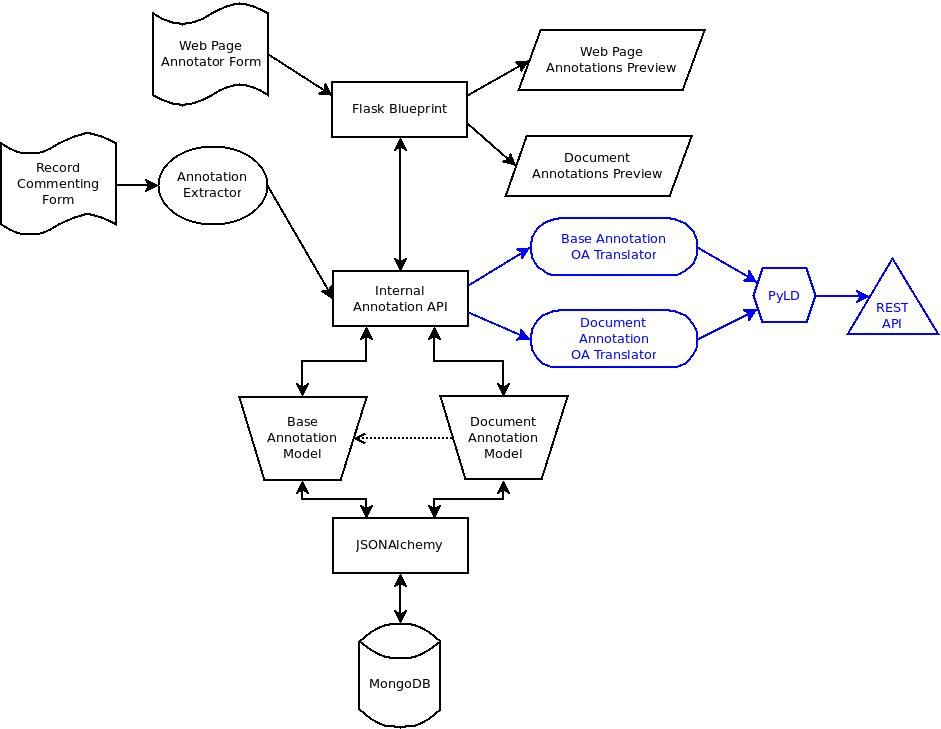
\includegraphics[scale=0.490]{static/dia/rest_anno.jpeg}}
  \caption[Annotation dissemination workflow]
          {Annotation dissemination workflow; after being translated to a proper
           standardised format (Open Annotation JSON-LD) and processed by PyLD,
           user-added annotations can be served by the Invenio REST API to
           concerned third-parties.}
  \label{fig:restanno}
\end{figure}


  \clearpage

  \section{Conclusions and Future Directions}
    \label{sec:outro}
    %!TEX root=../../main.tex

FIXME: wiki usecases, XTiger form, note validator (hierarchy, syntax), import
annotations from other (web)apps (e.g., Adobe)
FIXME: add annos by REST


  \bibliographystyle{alpha}
  \bibliography{bib/myrefs}

  \appendixpage
  \addappheadtotoc

  \appendix
    \section{Open Repositories 2014 Paper Submission}
      \label{apx:or2014}
      %!TEX root=../../main.tex

\paragraph{OR'2014} This appendix contains the paper submitted to the $9^{th}$
International Conference on Open Repositories (OR'2014), taking place in
Helsinki, Finland. It is the leading conference in its field, with hundreds of
participants from all around the world. The website of the conference is
\url{http://or2014.helsinki.fi/}.

Note that this paper was authored approximately two months before the end of
the project, and thus, certain details might be missing or inaccurate in
regards to the final state of the deliverable.

Paper follows on next page, the length being of three pages.

\paragraph{AAHEP7} A presentation regarding the annotation developments in
Invenio will be given by Dr. Tibor \v{S}imko at the $7^{th}$ Summit of
Information Providers in Astronomy, Astrophysics and High Energy Physics. This
summit is attended by representatives of organisations providing access to
information in these fields, such as INSPIRE, ADS or arXiv, and major
publishers such as the American Institute of Physics (AIP), American Physical
Society (APS), Elsevier, Institute of Physics (IOP) or Springer. It will take
place at the Stony Brook University, Stony Brook, New York, United States of
America, between 1--3 April, 2014. The event's website is
\url{http://indico.cern.ch/event/262430/}.

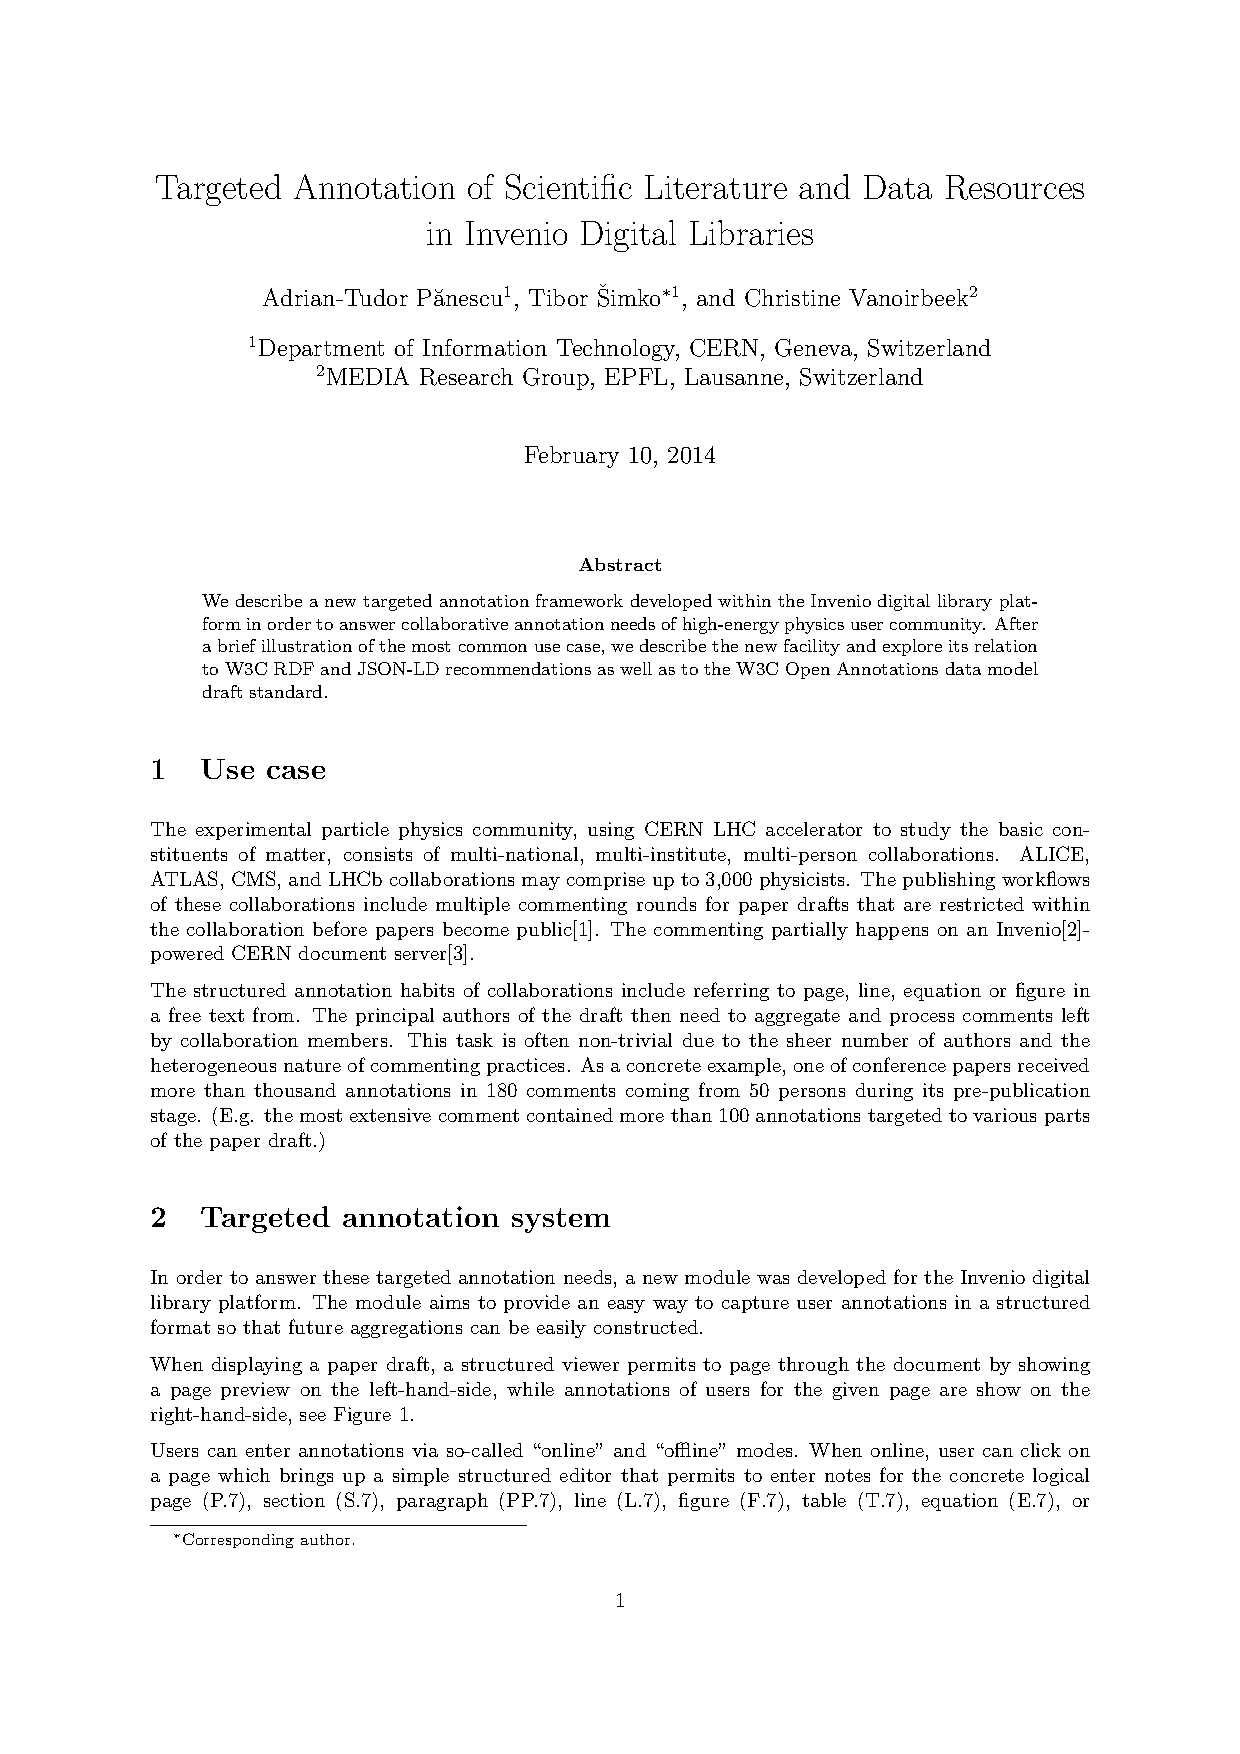
\includepdf[pages={1-3},frame=true,noautoscale=true,scale=0.85]{static/pdf/or2014-invenio-annotations.pdf}


    \section{Source Code Contributions}
      \label{apx:code}
      %!TEX root=../../main.tex

This appendix summarises the source code deliverables of the project.

All contributions of the project have already been merged for inclusion in
the next version of Invenio, and can be found online at
\url{http://invenio-software.org/repo/personal/invenio-apanescu}. Note that the
\texttt{pu} (\textit{``Proposed Updates''}) branch refers to the next Invenio
version, while the \texttt{labs} branch is used for the Invenio Labs
demonstrator.

As recorded by the Git source code control system, 79 commits, with 5948
additions and 1770 deletions were delivered. Out of these, 6 commits, with
3431 additions and 182 deletions, represent the annotation facilities, along
with the document previewer and other auxiliary components.

At \url{http://github.com/adrianp/invenio-demosite} the contributions
brought to the separate package used for deploying customised Invenio
installations can be found. Of interest is the \texttt{labs} branch, used for
Invenio Labs.

Two external software libraries have been maintained in order to fit the
project's requirements. These are PyLD (\url{http://github.com/adrianp/pyld}),
which was patched in order to function with the Python 2.6 version used for
Invenio Labs (see \texttt{python2.6} branch), and Intro.js
(\url{http://github.com/adrianp/intro.js}), a JavaScript library used for the
Invenio Labs interactive tutorial feature (see \texttt{inveniolabs} branch).
A bug fix for Intro.js has been accepted by the library authors and merged
upstream (see \url{http://github.com/usablica/intro.js/pull/236}).


\end{document}
